\section{Definisi GIS(GEOGRAPHICS INFORMATION SYSTEM)}
Sistem Informasi Geografis (SIG) adalah sebuah sistem yang dirancang untuk menangkap, menyimpan, memanipulasi, menganalisa, mengatur, dan menampilkan seluruh jenis data geografi. SIG tidak lepas dari data spasial, yang merupakan sebuah data yang mengacu pada posisi, obyek, dan
hubungan di antaranya dalam ruang bumi. Data spasial dalam SIG terbagi menjadi dua model data
yaitu model data vektor dan model data raster. Model data vektor merepresentasikan bumi sebagai
suatu mosaik yang terdiri atas garis (arc/line), polygon (daerah yang dibatasi oleh garis yang
berawal dan berhenti pada titik yang sama),titik/point (node yang mempunyai label), dan nodes
(merupakan titik perpotongan antara dua buah garis).
Model data raster atau sel grid merepresentasikan obyek geografis sebagai struktur sel grid yang diwakili oleh setiap pixel pada citra. Model data raster sangat baik untuk merepresentasikan batas-batas yang berubah secara gradual seperti jenis tanah, vegetasi, dan lain-lain

\section{Definisi Data Spasial (GEOGRAPHICS INFORMATION SYSTEM)}
Data Spasial Sistem Informasi Geografis (SIG) model data yang akan digunakan dari bentuk dunia nyata harus dapat diimplementasikan ke dalam basisdata. Data ini dimasukkan ke dalam komputer yang nantinya memanipulasi objek dasar yang memiliki atribut geometri (entity spasial/entity geografis) 
(Prahasta, 2002a). Data spasial pada dasarnya dapat disimpulkan bahwa data spasial merupakan suatu entitas data dalam Sistem Informasi Geografis (SIG) yang dapat dikelola, dianalisa dan dapat memetakan informasi objek keruangan beserta data-data atributnya serta dapat disimpan di dalam database yang dapat ditampilkan kedalam suatu sistem tertentu sehingga dapat mendukung dalam pengambilan keputusan. 

\subsection{ABSTRAK}
Diagram  Voronoi merupakan konsep interdisipliner yang telah diterapkan pada berbagai bidang. Dalam sistem informasi geografis (GIS), kemampuan yang ada untuk menghasilkan diagram Voronoi biasanya fokus pada hal biasa (tidak berbobot) titik fitur/point (tidak linear atau area). Untuk integrasi yang lebih baik dari model diagram Voronoi dan GIS, pendekatan berbasis raster dikembangkan, dan dilaksanakan mulus sebagai perpanjangan ArcGIS menggunakan ArcObjects. Dalam tulisan ini, metodologi dan pelaksanaan ekstensi dijelaskan, dan contoh yang disediakan untuk fitur titik(point), line, dan poligon. Keuntungan dan keterbatasan ekstensi juga dibahas. Ekstensi memiliki beberapa fitur berikut: 
\begin{enumerate}
\(1) bekerja untuk titik, garis, dan fitur vektor poligon; 
\(2) dapat menghasilkan kedua diagram Voronoi biasa dan multiplicatively tertimbang dalam format vektor; 
\(3) dapat menetapkan atribut non-spasial fitur input ke Voronoi sel melalui bergabung spasial;
\(4) dapat menghasilkan biasa atau Euclidean dataset raster jarak tertimbang untuk aplikasi pemodelan spasial. Hasil dapat dengan mudah dikombinasikan dengan GIS dataset lain untuk mendukung analisis spasial berbasis vektor dan pemodelan spasial berbasis raster.

\subsection{Diagram Voronoi untuk Point, Line dan Poligon dalam fitur GIS}
	Mengingat satu set jumlah terbatas titik berbeda di ruang 2-D Euclidean, diagram Voronoi titik set adalah kumpulan dari daerah yang membagi pesawat, dan semua lokasi di satu wilayah (kecuali pada batas wilayah) lebih dekat ke titik sponding corre- daripada titik lain (Gbr. 1). Diagram Voronoi dinamai matematikawan Rusia Georgy Fedoseevich Voronoi yang didefinisikan dan mempelajari kasus n-dimensi umum pada tahun 1908. Diskusi tentang konsep diagram Voronoi dari titik pandangan-sejarah dan geometris dapat ditemukan di Okabe et al. (1992, 2000).
	Diagram Voronoi telah banyak diterapkan untuk masalah partisi ruang dalam berbagai disiplin ilmu, dari astronomi untuk geografi untuk zoologi. Okabe et al. (2000) tercatat 22 bidang di mana aplikasi diagram Voronoi dapat ditemukan, dan diyakini bahwa bidang aplikasi tidak terbatas pada daftar. Contoh aplikasi terbaru dari diagram Voronoi termasuk berbasis Voronoi selular automata (Shi dan Pang, 2000), tomografi adaptif 3-D di (. Bo Hm et al, 2000) geofisika prospeksi, analisis distribusi gempa bumi-dan peringatan dini.

\ref{point} Sebuah Gambar Voronoi Diagram Point.
\begin{figure}[ht]
	\centerline{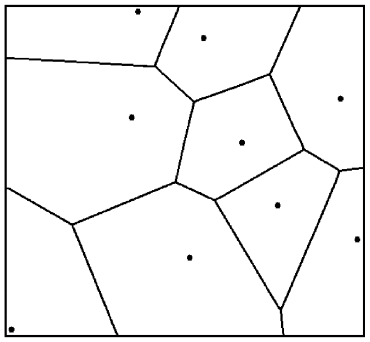
\includegraphics[width=1\textwidth]{figures/voronoi.PNG}}
	\caption{voronoi.}
	\label{voronoi}
	\end{figure}

\subsection{Model data Vektor pada Geographics Information System GIS}
Vektor  pada GIS mampu melakukan penempatan, menampilkan data spasial bahkan menyimpan datanya yang menggunakan titik-titik, garis-garis dan juga poligon yang dilengkapi dengan artibut-artibutnya. Bentuk-bentuk dasar representasi dari data spasial ini di dalam sistem model data vektor dapat didefinisikan oleh sistem koordinat kartesian dua dimensi (X,Y). Dimana di dalam model data spasial vektor, garis-garis atau kurva (busur atau arcs) adalah berupa sekumpulan titik-titik terurut yang saling berhubungan (Prahasta, 2002a). 

\subsubsection{Model data Vektor dengan bentuk point/titik pada Geographics Information System GIS}
Point/titik merupakan representasi grafis yang paling sederhana pada suatu objek. titik pada data vektor tidak mempunyai dimensi tetapi bisa ditampilkan ke dalam bentuk simbol baik pada peta maupun dalam layar monitor. contoh  lokasi fasilitas kesehatan, kantor pemerintah dan lain-lain.
Pada gambar \ref{point} dijelaskan bahwa gambar point/titik data vektor GIS sebagai berikut.
\begin{figure}[ht]
	\centerline{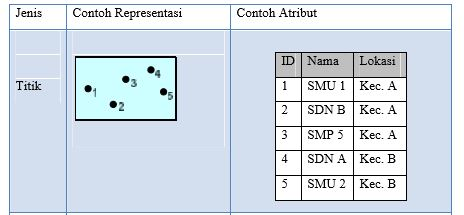
\includegraphics[width=1\textwidth]{figures/point.JPG}}
	\caption{point.}
	\label{point}
	\end{figure}

Maka artikel :
	Dalam sebuah artikel dari husein yang menyebutkan bahwa  GIS merupakan pemahaman dari
	Geography, Information dan System \cite{widiatmoko2009aplikasi}.

\section{contoh perancangan sistem (GEOGRAPHICS INFORMATION SYSTEM) dengan menggunakan Point}
Pada Point dapat menampung SHP yang bertipe Point.
Pada gambar \ref{kelaspoint} dijelaskan bahwa gambar point/titik data vektor GIS sebagai berikut.
\begin{figure}[ht]
	\centerline{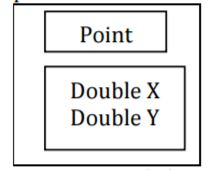
\includegraphics[width=1\textwidth]{figures/kelaspoint.JPG}}
	\caption{kelaspoint.}
	\label{kelaspoint}
	\end{figure}
Dimana didalam kelas terdapat artibut berupa :
\begin{enumerate}
\item X bertipe double, adalah titik koordinat dalam garis X dari sebuah point.
\item Y bertipe double, adalah titik koordinat dalam garis Y dari sebuah point.
\end{enumerate}
\subsection{Layer objek/point}
Dimana Layer dari sebuah point dapat dilihat dari gambar \ref{layerpoint}
 \begin{figure}[ht]
	\centerline{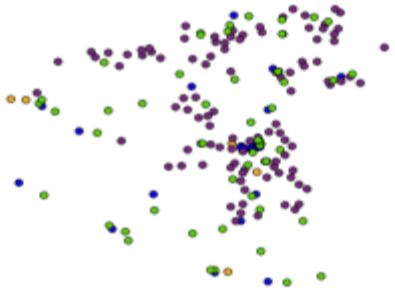
\includegraphics[width=1\textwidth]{figures/layerpoint.JPG}}
	\caption{layerpoint.}
	\label{layerpoint}
	\end{figure}
tipe data yang digunakan merupaka tipe data point yang terdapat koordinat real, yaitu berupa latitude dan longtitude. dimana layer ini mengkonfirmasi letak sekolah dan perumahan.

\subsection{Pola Titik}
	Pola titik (point pattern) adalah pola yang muncul dari sebuah variabel yang dianalisis pada daerah yang tersampel (Cressie, 1993). Sampel yang digunakan merupakan sebuah sampel yang memiliki bentuk tidak beraturan atau juga sampel yang memiliki jarak berbeda. Daerah tersebut dapat diperoleh dari sebuah data koordinat kartesius (x,y) dengan berdasarkan titik yang diamati. Data pada pola titik spasial yang sudah ada dapat diperoleh dari informasi apakah pola yang tadi diperoleh dapat menggambarkan keteracakan data spasial, clustering, ataupun keteraturan. Seperti contohnya yaitu : Penentuan sebuah posisi pohon-pohon yang memiliki ukuran tertentu. Apakah pohon-pohon tersebut dapat membentuk sebuah pola keteracakan spasial, clustering, ataupun keteraturan. Analisis dari data pola titik yang dilakukan karena agar dapat mengetahui apakah daerah titik yang akan menjadi objek penelitian tersebut membentuk daerah beraturan atau tidak , Sehingga nantinya dapat diketahui apakah terjadi ketergantungan antar titik atau tidak.   
	Pada estimasi dari data spasial, adalah teknik analisis data geostatistika bertujuan untuk mengetahui serta untuk melakukan estimasi nilai dari variabel teregional pada lokasi s. Nilai dari suatu variabel yang diamati nantinya dapat dinyatakan sebagai variabel random spasial  Z(s) dengan s adalah vektor lokasi D € R^d. Dan menggunakan metode kriging ini merupakan metode untuk melakukan estimasi nilai dari variabel yang teregional Z(s) pada suatu lokasi  A. berdasarkan variabel random spasial Z(s). Variabel random spasial  Z(s) pada data geostatistika merupakan suatu variabel random  Z di lokasi s . 
	Pada data spasial variabel random X dapat didefinisikan sebagai variabel random spasial Z(s) di lokasi  s dan dari variabel random Y didefinisikan sebagai variabel random spasial  Z(s+h) di lokasi s+h.  Pada analisis data geostatistika variansi ini digunakan untuk menentukan korelasi antara variabel random spasial Z(s) dan Z(s+h). Nilai variansi dari variabel random spasial pada lokasi Z(s) dan Z(s+h) dapat ditentukan dengan rumus sebagai berikut:
	var{z(s)  z(s+h)} = var{z9s0} + var{z(s+h)} 2cov{z(s).z(s+h)}
			    = E{Z(s)-z(s+h)}-{{E(z(s))-E(Z(s+h))}]


\subsection{MongoDB}
	MongoDB merupakan sebuah DBMS non relasional yang berorientasi dokumen dan bersifat open source yang ditulis dalam C++. MongoDB dikembangkan oleh perusahaan 10gen. Sebuah basis data pada MongoDB berisi satu atau lebih collections dari documents. Documents pada MongoDB dapat berisi nilai yang nilai tersebut dapat berisi sebuah document lain, kumpulan document, atau tipe data dasar seperti Double, String, dan Date. MongoDB menyiapkan tipe pengindeksan geospasial yang berguna mendukung keperluan kueri geospasial seperti 2D dan 2DSphere. Indeks 2D digunakan untuk menyimpan data sebagai titik pada bidang datar dua dimensi. Sedangkan apabila titik tersebut disimpan pada bidang lengkung maka indeks 2DSphere dapat digunakan. Secara default, sistem referensi koordinat yang digunakan MongoDB pada objek lengkung seperti bumi yaitu WGS84. MongoDB mendukung tipe data geospasial seperti Point, LineString, Polygon, MultiPoint, MultiLineString, MultiPolygon, Feature, FeatureCollection, dan GeometryCollection (de Souza etal. 2014).

Membuat Data Geospasial
Import shapefile
Masukan variable, misalkan variable a untuk shapefile.writer( )
a = shapefile.writer( )
Jadi, format membuat data geospasial ada 2, yaitu :
.shp => a.point(x,y)
a.poly [(x,y),(v,w)]
.dbf => a.field (‘name.field’,’c’,’40’)
a.record (‘bdg’)
Data geospasial tersebut disimpan menggunakan method a.save(‘file.shp’).

Arti dari method pada writer :
Point (x,y)	: memasukkan data berbentuk paint ke dalam .shp dan seluruh data harus  berformat ESRI.1
Poly [(a,b),(c,d)]	: memasukkan data geospasial berbentuk polygon (kembali ke titik    awal) atau polyline (tidak kembali ketitik awal).
Field (‘nama’,’c’,’40’)	: artinya membuat atribut polygon dengan table ‘nama’ dengan tipe data varchar dengan panjang 40. Method ini dapat diulang dan dapat dilakukan untuk krbuthan field baru lagi.
Record(‘Bandung’)	: Mengisi table dimana yang hanya 1 field dengan value atau nilai    ‘Bandung’.
Save (‘file name’)	: menyimpan file dengan save file

	Titik(dimensi nol - point) adalah representasi grafis atau geometri yang paling sederhana bagi objek spasial. Representasi ini tidak mempunyai dimensi, namun di atas peta dapat di identifikasikan lalu dapat di tampilkan pada layar monitor dengan menggunakan simbol-simbol tertentu. Perlu dipahami juga bahwa skala peta akan menentukan apakah suatu objek akan ditampilkan sebagai titik atau polygon. Pada peta yang berskala besar, unsur unsur bangunan akan di tampilkan sebagai polygon, sedangkan pada skala kecil akan ditampilkan sebagai unsur-unsur titik.
Format titik : koordinat tunggal, tanpa panjang, tanpa luasan.
Contoh : lokasi kecelakaan, letak pohon

